\documentclass{beamer}

% See this: http://texblog.net/latex-archive/uncategorized/beamer-warnings/
\let\Tiny=\tiny

\usepackage[
    compress,
    %minimal,
    %nonav,
    red,
    %gold,
    blue,
    %numbers,
    %nologo,
    %nominilogo,
    minilogoleft,
    polyu,
    comp,
    forty,
    %seventyfive,
]
{beamerthemeHongKong}

\title[Title short]{Title full}
\author[Author short name]{Author full name}
\institute[institute]{institute full name}
\date{\today}

\begin{document}

\frame{\titlepage}

\section*{Table of Contents}
\frame {
  \frametitle{\secname}
  \tableofcontents
}

\AtBeginSubsection[] {
  \frame<handout:0> {
    \frametitle{Outline}
    \tableofcontents[current,currentsubsection]
  }
}

\section{Section A}

\subsection{Subsection A-A}

\begin{frame}{\subsecname}
  \begin{columns}
  \column{0.5\textwidth}
    \begin{figure}
    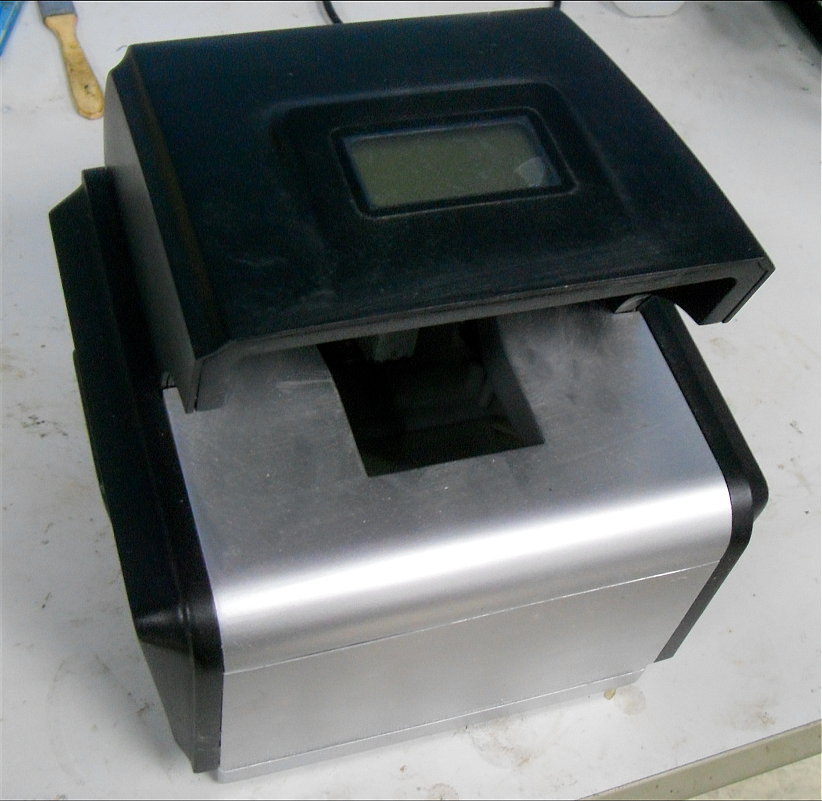
\includegraphics[width=\textwidth]{image/test-image1}
    \caption{figure A}
    \end{figure}
  \column{0.5\textwidth}
    \begin{block}{example}
      \begin{enumerate}
        \item<alert@1>
        text about figure A
        \item
        text
      \end{enumerate}
    \end{block}
  \end{columns}
\end{frame}

\subsection{Subsection A-B}

\section{Section B}

\section{Section C}

\subsection*{Thanks}

\begin{frame}{\subsecname}
  \begin{columns}
  \column{2.5cm}
  \column{5cm}
    \Huge{Thank you!}
  \column{2.5cm}
  \end{columns}
\end{frame}


\end{document}
